%% Copernicus Publications Manuscript Preparation Template for LaTeX Submissions
%% ---------------------------------
%% This template should be used for copernicus.cls
%% The class file and some style files are bundled in the Copernicus Latex Package, which can be downloaded from the different journal webpages.
%% For further assistance please contact Copernicus Publications at: production@copernicus.org
%% https://publications.copernicus.org/for_authors/manuscript_preparation.html


%% Please use the following documentclass and journal abbreviations for preprints and final revised papers.

%% 2-column papers and preprints
\documentclass[hess, manuscript]{copernicus}

\usepackage{inputenc}
\usepackage{url}
\usepackage{graphicx}
\usepackage{adjustbox}
\usepackage{amssymb}
\usepackage{amsfonts}
\usepackage{amsmath}
\usepackage{nicefrac}
\usepackage{microtype}
\usepackage{hyperref}
\usepackage{ulem}
\usepackage{enumitem}
\usepackage{float}
\usepackage{datetime}
\usepackage{xkeyval}
\usepackage{framed}
\usepackage{pdflscape}
\usepackage{booktabs}
\usepackage{longtable}
% template
\usepackage{fancyvrb}
\usepackage{mathtools}

% colors for hyperlinks
\hypersetup{colorlinks=true, allcolors=blue}

\begin{document}

\title{Recession analysis of a steep slope watershed: the fast and slow flow compartmentalization of the Kahule Khola catchment (Nepal, Himalaya)}

\Author[1]{John}{J. Armitage}
\Author[1,2]{Kapiolani}{Teagai}
\Author[1]{Léo}{Agelas}
\Author[2]{Niels}{Hovius}
\Author[3]{Christoff}{Andermann}

\affil[1]{IFP Energies Nouvelles}
\affil[2]{GFZ Potsdam}
\affil[3]{OSUR, Université Rennes}

%% The [] brackets identify the author with the corresponding affiliation. 1, 2, 3, etc. should be inserted.

%% If an author is deceased, please mark the respective author name(s) with a dagger, e.g. "\Author[2,$\dag$]{Anton}{Smith}", and add a further "\affil[$\dag$]{deceased, 1 July 2019}".

%% If authors contributed equally, please mark the respective author names with an asterisk, e.g. "\Author[2,*]{Anton}{Smith}" and "\Author[3,*]{Bradley}{Miller}" and add a further affiliation: "\affil[*]{These authors contributed equally to this work.}".

\correspondence{John J. Armitage (john-joseph.armitage@ifpen.fr)}

\runningtitle{Ubiquitous weathering}

\runningauthor{Armitage}

%% These dates will be inserted by Copernicus Publications during the typesetting process.
\received{}
\pubdiscuss{} %% only important for two-stage journals
\revised{}
\accepted{}
\published{}

\firstpage{1}

\maketitle

\begin{abstract}
Text
\end{abstract}

\section{Introduction}

Mountains have long been recognized as vital reservoirs of freshwater, with most of the rivers in the world originating in these high elevation regions. In the early 2000s, initiatives such as The Abisko Agenda: Research for Mountain Area Development began to highlight the importance of mountain groundwater with the still undergoing context of climate change, emphasizing the critical roles as sources of biodiversity and freshwater for supplying surrounding lowlands \citep{abisko-2002,viviroli-2004}. Despite their importance as subsurface storage zones, mountain catchments display a range of hydrological responses to water inputs. These responses are strongly influenced by the geomorphological and geological characteristics of the terrain, which determined how water is partitioned, stored, and subsequently released within or across compartments \citep{beven-1982}.

In steep mountain environments, particularly in tectonically active regions such as the Himalayas, the interplay between water input and hydrological response is highly complex. The inherent steepness and ongoing uplift in these regions fundamentally drive the processes of infiltration, storage, and discharge \citep{montgomery-2003}. \cite{clarke-2011} emphasized that the topographic gradients and active geological processes not only facilitate rapid runoff but also influence the development of subsurface storage zones. For example, water that infiltrates through fractures and weathered rock may quickly contribute to stream flow, while water stored in deeper or more confined compartments can be released over extended periods \citep{beven-2012}.

Field studies in the Nepal Himalayas further illustrate this complexity. \cite{andermann-etal-2012} documented groundwater response times on the order of 45 days in fractured basement aquifers, highlighting the temporal lag between precipitation or snow melt inputs and groundwater contributions to stream flow. Such delayed responses confirm the non-linear and compartmentalized nature of subsurface hydrological dynamics in steep mountain catchments. \cite{chatton-2017} observed rapid and time-lagged variations in baseflow chemistry, suggesting multiple groundwater flow compartments within fractured Himalayan aquifers. However, the actual mechanisms controlling subsurface water circulation remain poorly understood. In fractured subsurface environments, it is possible that fractures act as preferential flow paths, offering significantly higher permeability than the surrounding matrix \citep{rempe-2018}. Similarly, \cite{somers-2020} emphasized that steep mountain systems often contain both near-surface weathered zones and deeper fractured reservoirs, each contributing to stream flow at different timescales.

In humid areas, the contribution of mountain to total discharge generally does not exceed 50\,\% but can easily exceed 50\,\% in arid or semi-arid areas \citep{messerli-etal-2004}. The hydrological significance of mountain regions is an indicator of the role of the subsurface as a modulator of the runoff response. For a long time, it was assumed that lateral subsurface storm flow was the primary runoff generating mechanism along the soil-bedrock interface \citep{weiler-etal-2006}. Then, numerous studies shown that the bedrock compartment can also be a significant discharge component \citep{katsuyama-etal-2009,tromp-van-meerveld-etal-2007}. The recent works of \cite{rempe-2018} have demonstrated that the bedrock underlying steep mountain regions consists of distinct compartments formed by variations in term of weathering intensity (fracture sizes, inter-connectivity) and lithological distribution. If the lateral extension of the weathered zone is indicative of the control on subsurface storm flow from hillslope and runoff \citep{jencso-etal-2009,tromp-van-meerveld-2006}, recent findings suggest that the vertical and widespread extension of the weathered zone can also play the role of a buffer in the Himalayas \citep{teagai-etal-2026}, storing temporarily groundwater at the onset of monsoon before releasing when the peak of precipitation is reached. These differences give rise to varied hydrological behaviours within the same hillslope according to the geological, lithological, and climatic conditions.


\subsection{Weathering zone in the Bhota Koshi}

In Nepal, the climate is strongly influenced by the Indian Summer Monsoon (ISM), which produces a distinct seasonal cycle characterized by a long-wet season (March–November) and a short-dry season (December–February). In central Nepal lies the Bhote Kosi basin, a typical Himalayan basin that drains both the Lesser and High Himalayas. This watershed receives approximately 80\,\% of its annual rainfall during the ISM season . Before the onset of the monsoon, sporadic and intense rainfall originating from the plains south of the Himalayas deliver significant volumes of water and effectively pre-conditioning the weathered zone . Under such climatic conditions, the capacity of the subsurface to store and redistribute water becomes critical.

Recent studies in the Bhote Kosi basin, using seismic interferometry and a combined method encompassing geophysical, hydrological and spring chemistry data, have demonstrated that the weathered zone acts as a buffer at the onset of wet season \citep{illien-etal-2021,teagai-etal-2026}. In pre-monsoon, the weathered zone modulates the rainfall infiltration rate and groundwater transfers to deeper aquifers. Seismic velocity analyses across different sites reveal that the weathered zone is highly sensitive to local geological and hydrological conditions, reinforcing its function as a modulator to groundwater systems. In this area, although fractures influence the groundwater preferential flow paths along the surface-bedrock interface, the widespread weathered zone stores temporarily groundwater in at least the first 20 m depth \citep{teagai-etal-2026}. Once the storage capacity is exceeded, excess water moves into deeper aquifers. The model fit to $dV/V$ from seismic interferometry suggest a buffering effect of evapotranspiration within the weathering zone \citep{illien-etal-2021}. ERT transects indicate a change in saturation within a well defined topmost layer down to 20\,m depth within various morphological land types, from gullies to ridges. The question remains as to if this weathering zone and hence compartmentalisation of the hydrogeologic response is systematic across the landscape and how it impacts groundwater storage and release.

\subsection{Recession curves and insights into aquifer response}

To understand the hydrological response of the mountain catchment system to changes in water input we will focus on recession analysis. Recession analysis is performed by plotting the time rate of change in discharge $-dQ/dt$ versus discharge $Q$ in a log-log space. These resulting recession curves, which depict the decline in river discharge over time following a storm event or snow melt, capture how the catchment returns to its baseflow conditions. The shape and slope of these recession curves provide insights into the spatial integrated and temporal variability of hydrological processes across the compartmentalised subsurface \citep[e.g.][]{roques-etal-2022}. 

The falling limb of the recession curve can be modelled by a power-law relationship between the time rate of change in discharge as a function of discharge \citep[e.g.][]{brutsaert-1977,kirchner-2009},
\begin{equation}
-\frac{dQ}{dt} = aQ^{b}
\label{eq:recession}
\end{equation}
with $a$ and $b$ representing the geometric and hydraulic characteristics of the groundwater system. In particular, the parameter $b$ characterizes the non-linearity relationship between the storage and the river discharge, often referred to as the storage-discharge function. The recession can be split into the initial \emph{fast} response and the later \emph{slow} response. Model derived slow response from the Dupuit-Boussinesq aquifer model has a $b$ of 1 or 1.5 depending on the length of the groundwater system \citep{brutsaert-1977}. If the water table does not vary significantly during recession, e.g. the system is very large, then the recession will follow an exponential decay and $b=1$ \citep{brutsaert-1977}. If however the aquifer is locally constrained then the recession will take the form of a power law, and under the assumptions of the Dupuit-Boussinesq model $b=1.5$.

A compilation of stream flow recession analysis for the USA however found that in mountain environments the recessions do not fit the Dupuit-Boussinesq model with $b=1$ to 1.5 \citep{tashie-etal-2020}. Higher values of $b$ for the slow flow in steep topography have been generated for compartmentalised domains, with a top subsurface layer that has high hydraulic conductivity above a deeper low conductivity layer \citep{rupp-2006,roques-etal-2022}. For slow flow, the upper limit in these models is of $b\sim2$. It has however been recognised that the early recession has a $b>1.5$. In the data set of recessions from the USA, early recession is consistently high \citep{tashie-etal-2020}. This high $b$ is most likely due to the transition from fast flow post rainfall to the slow flow that signifies drainage of the deeper aquifer. Numerical modelling of a compartmetalised groundwater system has suggested the $b$ will transition from values as high as 5 depending on the ratio of hydraulic conductivity and gradient \citep{roques-etal-2022}.

\section{The Kahule Khola subcatchment}

\begin{figure}
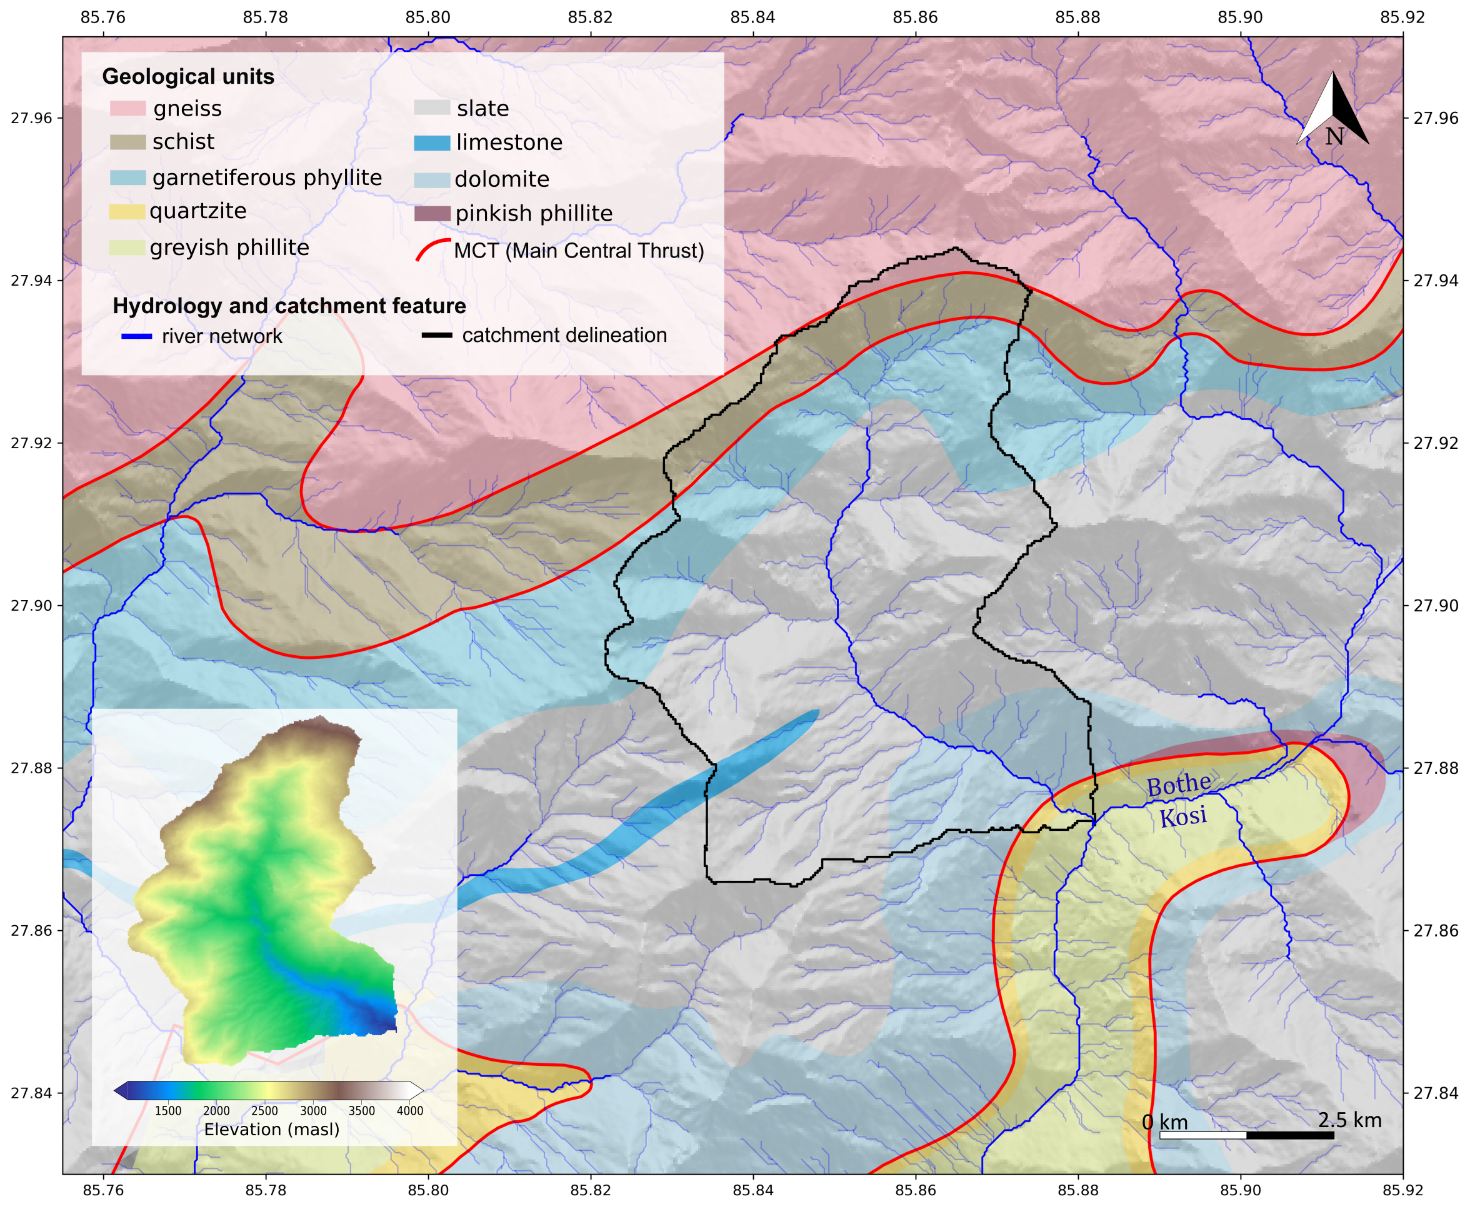
\includegraphics[width=.8\linewidth]{./figures/figure01.png}
\caption{Map elevation in 3D of the Kahule Khola catchment, a tributary of the Bhote Kosi River, located at the junction of the Lesser Himalaya and the Great Himalayan Sequence delineating the active Main Central Thrust (MCT).}
\label{fg:location-map}
\end{figure}

The Kahule Khola watershed, a tributary of the Bhote Kosi River, is an unglaciated catchment located in central Nepal. The catchment, of surface area $33\rm\,km^{2}$, is situated at the junction of two geological zones within the Himalayan Mountain system: the Lesser Himalayas, composed of primarily of moderately metamorphic rocks (slate, phyllite, quartzite) and sedimentary rocks (limestone, dolomite) that have undergone significant folding and faulting; and the High Himalayas (also called Great Himalayan Sequence), composed of igneous and high-grade metamorphic rocks (gneiss, schist) that are the tectonic core of the Himalayan Mountain range. The Bhote Kosi basin is crossed by the Main Central Thrust (MCT), a shear zone where the High Himalayan range slid over the Lesser Himalaya to the north . Two strands of the MCT fault system cut through the Kahule Khola catchment. The junction delimits a primary strand forming the upper limit of the Lesser Himalayan formations, located around ~3300 masl, and a secondary strand located at ~1300 masl near the outlet of the catchment, separates the sedimentary and metamorphic formations within the Lesser Himalayan stack. With elevations ranging from 1076 masl to 3471 masl, the landscape is marked by rugged topography where steep slopes average 33\,$\deg$ (varying between 6\,$\deg$ and 66\,$\deg$) and are intermittently interrupted by remnant landslides where water carves its way through exposed bedrock, boulders, and colluviums, while feeding the hydrographic network. These geomorphic features are clear indicators of the ongoing tectonic activity in the region.

\cite{teagai-etal-2026} showed evidence of a weathering layer of 10 to 20\,m depth during monsoon that is then drained in post-ISM, and suggest that rainfall infiltrates in a continuous and widespread weathering layer before reaching groundwater with no overland flow. These observations agree with the findings of \cite{illien-etal-2021} from passive seismic monitoring in the area suggesting a buffer between infiltrating rainwater and its arrival to the deep groundwater. This has led to assume that there is a subsurface compartmentalization, consisting of a weathered layer which buffers the underlying less fractured bedrock reservoir, slowly releasing groundwater to sustain baseflow that maintains perennial stream flow during the dry season.

\section{Methods}

\subsection{Data acquisition}

As part of the PRESSurE Project conducted following the Gorkha earthquake in 2015, multiple data series were collected between June 2015 and October 2018 within the Bhote Kosi basin such as data series of precipitation and river stage height \citep{andermann-etal-2021}. Daily precipitation [mm] were collected from six meteorological stations distributed in and around the Kahule Khola catchment (Figure \ref{fg:location-map}). Based on the Polygon Thiessen method, the rainfall three weather stations (Gumba, Listi and Tyanghtali) are the most relevant to estimate the amount of rainfall within the Kahule Khola catchment. River stage height [m] was measured at the catchment outlet and observations were recorded every 5 minutes intervals. 

\begin{figure}
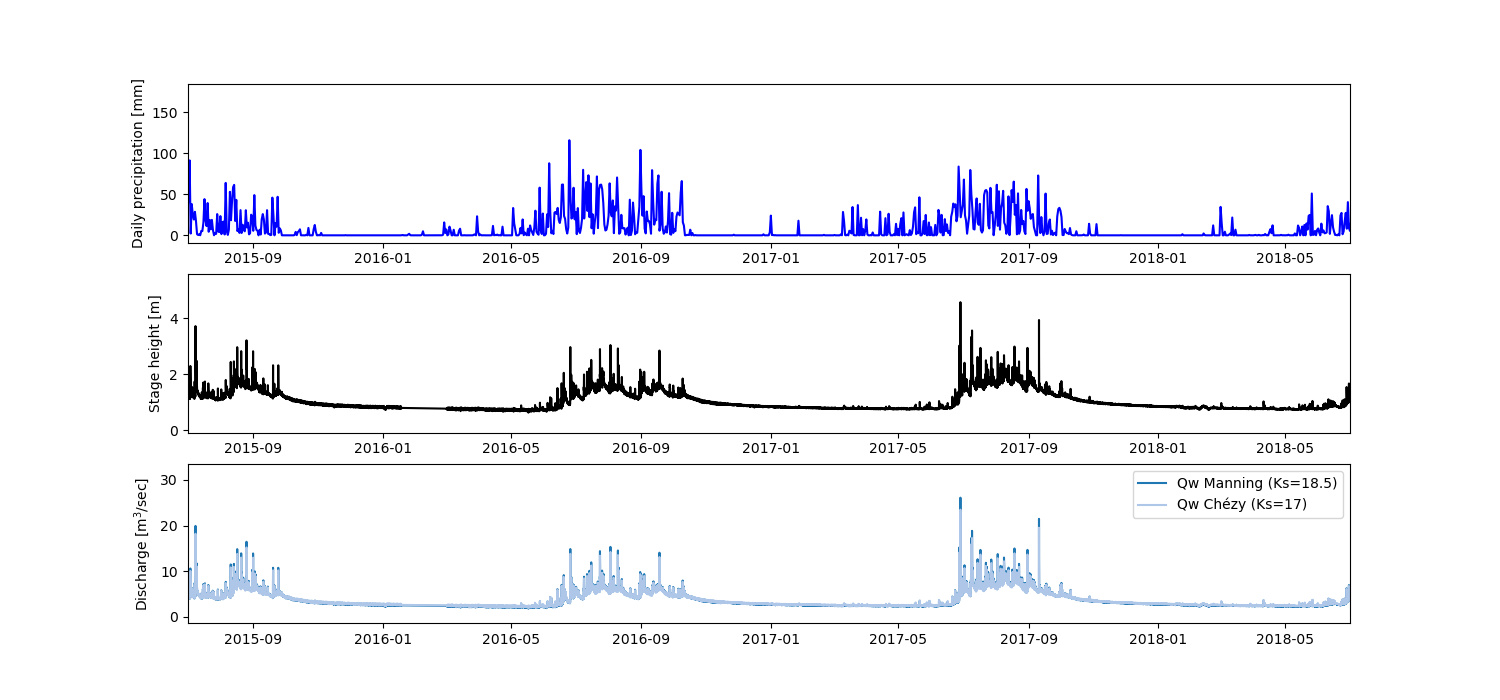
\includegraphics[width=1.\linewidth]{./figures/figure02.png}
\caption{Time series of daily precipitation (in blue) and river stage (in orange) averaged from daily values. Precipitation data were spatially weighted using the Thiessen polygon method based on three weather stations, while river stage height was measured at the outlet of the Kahule Khola catchment. The observations period span June 2016 to October 2018.}
\label{fg:rain2discharge}
\end{figure}

\subsection{Discharge estimation}

In Kahule Khola catchment, groundwater recharge occurs by monsoonal rainfall. To capture the spatial and temporal related storage dynamics of the catchment, we estimated the river discharge ($Q$) at the outlet using the Manning-Strickler equation,
\begin{equation}
Q = K_{S}AR_{h}^{3/2}S^{1/2}
\end{equation}
and the Chézy equation,
\begin{equation}
Q = K_{S}bh \sqrt{R_{h}S}
\end{equation}
where $S$ [-] is the friction slope of the riverbed, $A$ [m$^{2}$] is the channel cross-section area where the pressure gauge was deployed, $K_{S}$ [s\,m$^{-1/3}$ for Manning-Strickler or m$^{1/2}$s$^{-1}$ for Chézy] is the roughness parameter for each model, and $R_{h}$ [m] is the hydraulic radius. This equation relates the average water flow velocity of an open channel flow. The channel cross-section where the pressure gauge was deployed has a roughly rectangular shape which corresponds to a hydraulic radius,
\begin{equation}
R_{h} = \frac{bh}{b + 2h}
\end{equation}
where $b$ [m] is the width of the channel and $h$ [m] is the average river height. The channel width was measured as 2\,m  and we attributed a relatively flat local slope $S=0.02$. We varied values of $K_{S}$ for both models to obtain a reasonable river discharge relative to the total annual rainfall. Figure \ref{fg:rain2discharge} presents the mean daily discharge for the different tested values of $K_{S}$ for both the Manning-Strickler and Chézy models. Using the 2017 monsoon season to for a water balance, was approximately 3446\,mm of rainfall fell across the catchment. This results in a equivalent discharge of 3427\,mm for the Manning’s roughness coefficient occurs for $K_{S}=18.5$ or 3444\,mm for a Chézy coefficient of $K_{S}=17$ (Figure \ref{fg:rain2discharge}).

From the discharge time series we use the method of \cite{kirchner-2009} with the addition of a bootstrap method to estimate the recession characteristics and the uncertainty in the values for the three post monsoon seasons in our time series (Figure \ref{fg:rain2discharge}). First $dQ/dt$ is calculated along the time series and all values of $dQ/dt$, including positive values are sorted along with the corresponding value of $Q$. The data is then binned into bins defined by the logarithmic range of the data, where by bins are populated depending on if the standard error in the population of data points is less than half of the mean (including both positive and negative $dQ/dt$). For a full description of the binning algorithm see \cite{kirchner-2009}. 

We subsequently note that the data show a separation between trends for early and late recession, and split the binned data to run a linear regression. Linear regressions are run using a bootstrap method to asses the range of potential $b$. We make a repeat re-sampling of the binned data, removing a data point each time, to find the different potential fits to the recession analysis.

\subsection{Compartmentalized groundwater model}

Groundwater flow equations provide a conceptual framework of the physical processes governing subsurface water movement. One common approach to solving these equations involves estimating the pressure head $h_{p}$ at any point in the domain. Darcy’s law is the fundamental equation used to describe the flow of fluid through porous media. In an isotropic medium, in which material properties are uniform and independent of direction, the specific flow rate of water  $u_{w}$  is defined as a function of hydraulic conductivity and pressure head expressed as,
\begin{equation}
u_{w} = -KX(s_{e})\left(\nabla h_{p} + \hat{\mathbf{e}}{z}\right)
\end{equation}
where $K$ [LT$^{-1}$] is the hydraulic conductivity, $X(s_{e})$ is a relative permeability function depending on the amount of water into the subsurface, and $\hat{\mathbf{e}}_{z}$ is the unit vector in the upward vertical direction. The relative permeability function is dependent on the effective saturation, which is defined as,
\begin{equation}
s_{e} = \frac{\theta - \theta_{r}}{\theta_{s} - \theta_{r}}
\label{eq:se}
\end{equation}
where $\theta$ [-] is the volumetric water content, $\theta_{s}$ is the content at saturation, and $\theta_{r}$ is a reference content.

The conservation of water mass is then expressed by,
\begin{equation}
\frac{\partial \theta}{\partial t} + \nabla \cdot u_{w} = R
\end{equation}
$R$ [T$^{-1}$] is the source recharge term. We assume that the effective saturation is linearly related to the pressure head, given by,
\begin{equation}
s_{e} = c_{S}h_{p}
\end{equation}
where $c_{S}$ [L$^{-1}$] is the specific storage coefficient. Including this definition the volumetric water content is,
\begin{equation}
\theta = \left(\theta_{s} - \theta_{r}\right)c_{S}h_{p} + \theta_{r}
\label{eq:theta}
\end{equation}
The combination of the conservation of mass and Darcy's flow, and applying the chain rule \citep[e.g.][]{farthing-2017}, gives Richards equation in the form, 
\begin{equation}
\frac{\partial \theta}{\partial h_{p}}  \frac{\partial h_{p}}{\partial t} - \nabla\cdot\left[KX(s_{e}) \nabla\left(\nabla h_{p} + \hat{\mathbf{e}}_{z}\right)\right] = R
\label{eq:richards}
\end{equation} 

\subsubsection{Relative permeability function}

The closure term, or relative permeability function $X(s_{e})$, paramerterises how hydraulic conductivity varies with the saturation of the subsurface. In soils and saphrolite the Van Genuchten-Mualem model is commonly used. In this study we define a simpler functional form of $X(s_{e})$ that allows us to deal with flow through the deeper fractured bedrock layer, reduce the number of unknown parameters and reduce the computational cost. From combining our definition of $\theta(h_{p})$ (equation \ref{eq:theta}) and $s_{e}$ (equation \ref{eq:se}), it can be seen that $X(s_{e})$can be expressed as $X(h_{p})$. We subsequently express the effective saturation as a function of the pressure head $h_{p}$ (varying between 0 and 1),
\begin{equation}
X(s_{e}) \coloneqq X(h_{p}) =
\begin{cases} 
0, & \text{if } h_{p} \leq 0, \\
\left(C_{1}h_{p}\right)^{\gamma_{s}}, & \text{if } 0 < h_{p} < \frac{1}{C_{1}}, \\
1, & \text{if } h_{p} \geq \frac{1}{C_{1}}.
\end{cases}
\label{eq:closure}
\end{equation}
where $C_{1}$ [L$^{-1}$] is a storage parameter and $\gamma_{s}$ [-] is a shape parameter that modulates the curvature of the relative permeability function. $C_{1}$ defines the pressure head at which full saturation is reached. Lower values of $C_{1}$  shift the saturation point to higher values of $h_{p}$, mimicking materials that require stronger capillary tension to reach full saturation. Conversely, larger values of $C_{1}$ produce earlier saturation representing more permeable and coarser-textured soil. In contrast, $\gamma_{s}$ governs the shape and the non-linearity of the permeability response as a function of the saturation. As $\gamma_{s}$ increases, the function $X(h_{p})$ becomes more concave and the permeability remains low for a large part of unsaturated range before rising steeply near saturation. This behaviour mimics the hydraulic response of structured or compacted soils, where water flow remains limited until a threshold saturation is reached. By tuning $C_{1}$ and $\gamma_{s}$, it is possible to mimic the saturation thresholds and conductivity transitions seen in nonlinear models such as the Van Genuchten-Mualem model, while preserving computational simplicity.

\begin{figure}
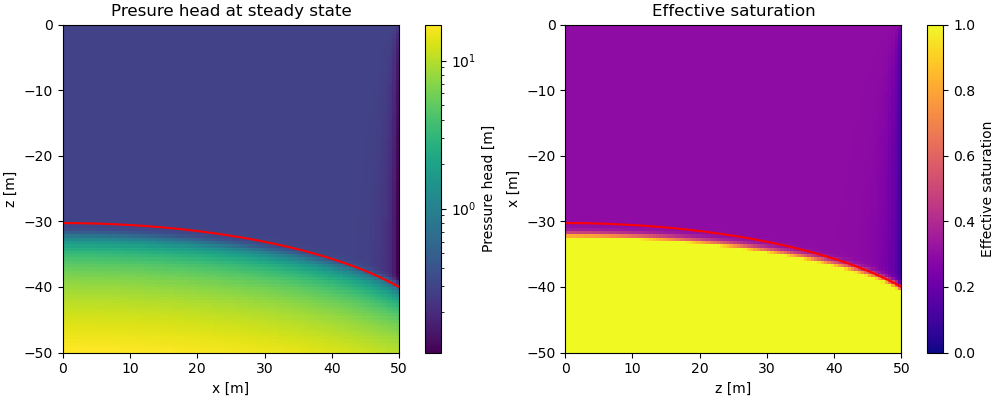
\includegraphics[width=0.8\linewidth]{./figures/figure03.png}
\caption{Pressure head and effective saturation at steady state for a Dupuit-Boussinesq model, where the top boundary is open. The left and bottom boundary are closed, and the water table is fixed at -40\,m on the right hand side. The analytic solution to the steady-state water table is plotted in red.}
\label{fg:steadystate}
\end{figure}

Our intention is to model the discharge of groundwater within the rock moisture layer that is typical of weathered bedrock and the the fracture bedrock aquifer below. To find an appropriate value for $C_{1}$ and $\gamma_{s}$ we search for values that generate a water table equivalent to the steady state Dupuit-Boussinesq model aquifer with a constant hydraulic conductivity of $K=10^{-5}\rm\,ms^{-1}$ and a fixed water table at the right hand side of 40\,m below the surface (Figure \ref{fg:steadystate}). We found that values of $C_{1}=1$ and $\gamma_{s}=2$ recover sufficiently the form of the steady state aquifer (Figure \ref{fg:steadystate}). We therefore use these values throughout the manuscript. 

\subsubsection{Initial conditions and parameters}

\begin{figure}
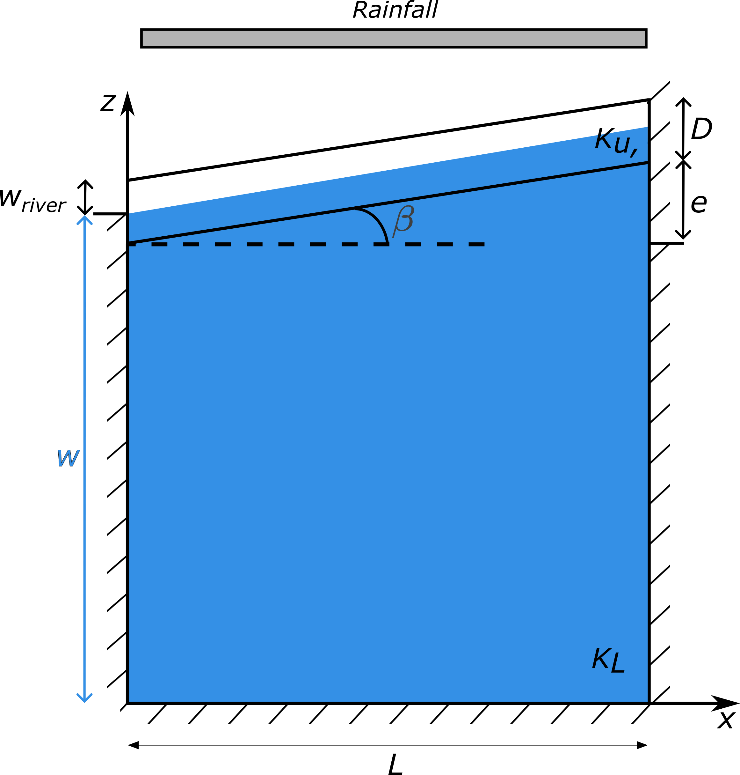
\includegraphics[]{./figures/figure04.png}
\caption{ Boundaries and initial conditions setting the model domain. The bottom and right boundaries are closed and no flow is allowed. The top of the domain is open and rainfall vertical exchanges (inflow/outflow) are allowed along the whole length. The left boundary is partially impermeable and flux are allowed to inflow and outflow in the top region defined by $w_{river}$.}
\label{fg:domain}
\end{figure}

We consider a 2D domain representing a sloping hillslope with a two-layered subsurface configuration, as shown in Figure \ref{fg:domain}, following the approach of \citep{roques-etal-2022}. The domain has a total horizontal length of 200\,m and comprises, an upper layer with a constant thickness $D$, hydraulic conductivity $K_{U}$ and saturated water content $\theta_{SU}$; a lower layer where the hydraulic conductivity $K_{L}$ and water content $\theta_{sL}$ decrease exponentially with depth according to \citep{cardenas-2010},
\begin{equation}
K_{L} = K_{0} exp\left[-\frac{1}{\alpha}\left(z_{s} - z\right)\right]
\end{equation}
and,
\begin{equation}
\theta_{sL} = \theta_{s0} exp\left[-\frac{1}{\alpha\eta}\left(z_{s} - z\right)\right]
\end{equation}
$z_{s}$ denotes the elevation of the interface between the upper and lower layers. This interface is parallel to the topography and follows a slope defined by a gradient $\beta$. The parameter $\alpha$ controls the rate at which hydraulic conductivity decreases with depth, while $\eta=2$ modifies $\alpha$ to governs the vertical decline of porosity \citep{roques-etal-2022}. This vertical heterogeneity allows the model to simulate the contrasting hydrodynamic behaviour of shallow and deep compartments, from a permeable weathered zone near the surface to a low permeable and less fractured bedrock at depth.

To test the hydrological sensitivity to structural parameters, following \cite{roques-etal-2022} we varied the gradient $\beta = [0.1, 0.2, 0.3]$, the thickness of the upper layer $D = [10, 20, 50]$, and the vertical hydraulic contrast $K_{U}/K_{L} = [16, 64, 256]$. For these simulations, we fixed the conductivity at the top of the lower layer $K_{0} = 5\times 10^{-6}\rm\,ms^{-1}$, and varied the upper conductivity as $K_{U} = [8\times 10^{-5}, 3.2\times 10^{-4}, 1.28\times 10^{-3}]\rm\,ms^{-1}$ . The porosity is assumed constant in the upper layer such as $\theta_{sU} = \theta_{s0} = 0.3$. A summary of all of the model parameters in in Table \ref{tb:parameters}.

\begin{table}
\caption{Model parameters}
\label{tb:parameters}
\begin{tabular}{c|c|l}
\toprule
Parameter & Value & Description \\
\hline
$\theta_{r}$ & 0 & Reference volumetric water content \\
$c_{S}$ & $5\times10^{-3}$ & Specific storage coefficient \\
$C_{1}$ & 0.1 & Closure equation storage parameter \\
$\gamma_{s}$ & 2.0 & Closure equation shape parameter \\
\hline
$\theta_{s0}$ & 0.3  & Saturated volumetric water content in the top layer \\
$K_{0}$ & $5\times 10^{-6}\rm\,ms^{-1}$ & Hydraulic conductivity of top of the lower model layer \\
$K_{U}$ & $8\times 10^{-5}\rm\,ms^{-1}$ & Hydraulic conductivity in the upper model layer \\
 & $3.2\times 10^{-4}\rm\,ms^{-1}$ & \\
 & $1.28\times 10^{-3}\rm\,ms^{-1}$ & \\
$\alpha$ & 100\,m & characteristic depth for decrease in hydraulic conductivity \\
$\eta$ & 2 & modifier for depth reduction in porosity (water volume content at saturation) \\
\end{tabular}
\end{table}

Boundary and initial conditions are defined such as bottom and right boundaries are impermeable (no flux). The left boundary is impermeable except in the topmost part, where above the depth $w_{river} = 10\rm\,m$ water is allowed to leave the domain (Figure \ref{fg:domain}. Vertical rainfall infiltration and overland flow are allowed at the top boundary. All precipitation is assumed to infiltrate into the subsurface and to be uniform along the whole length of the top boundary. The initial height of the water table is assumed to be 10\,m below the top surface and is parallel to the slopping interface. The numerical domain is discretised using trapezoidal cells with a maximum cell size of 2\,m by 2\,m, and the numerical solutions is found via a finite volume approach with Newton-Raphson iteration under variable hydraulic gradients.

To simulate a hydrological cycle representative of the Kahule Khola catchment, each model run spans 100 days and follows a two-phase rainfall forcing. During the first 50 days, a constant rainfall rate is applied to reproduce an annual input of 3500 mm. This intense and sustained recharge phase allows the system to reach dynamic saturation conditions. In the second half of the simulation (days 50 to 100), rainfall is abruptly stopped, and the model evolves in a free drainage regime, enabling the observation of natural depletion dynamics. This setup is specifically designed to isolate and analyse the recession behaviour of the system, particularly the discharge response and the evolution of the recession exponent $b$.

\section{Results and discussion}

\subsection{Recession analysis}

The 5 minute stage height data is converted to a discharge using the Manning-Strickler and Chezy model and subsequently the recession is analysed for the three post-monsoon seasons from 2016 to 2018. The two models to convert stage height to discharge give very similar trends for the recession analysis (Figure \ref{fg:recession}). The discharge magnitude is slightly higher with the Chézy model, however this is due to the choice of the roughness coefficient. The recessions are split into an early and late recession, where for the Manning Strickler model and Chézy model, the transition occurs at a discharge of $4.8\rm\,m^{3}s^{-1}$. From bootstrap re-sampling we find that the early recession $b$ is within the range $3.5 < b < 13.5$, with the two models overlapping in range (Figure \ref{fg:recession}). For the late recession the range is $2.4 < b < 3.2$ with a significant overlap in the two ranges (Figure \ref{fg:recession}).

\begin{figure}
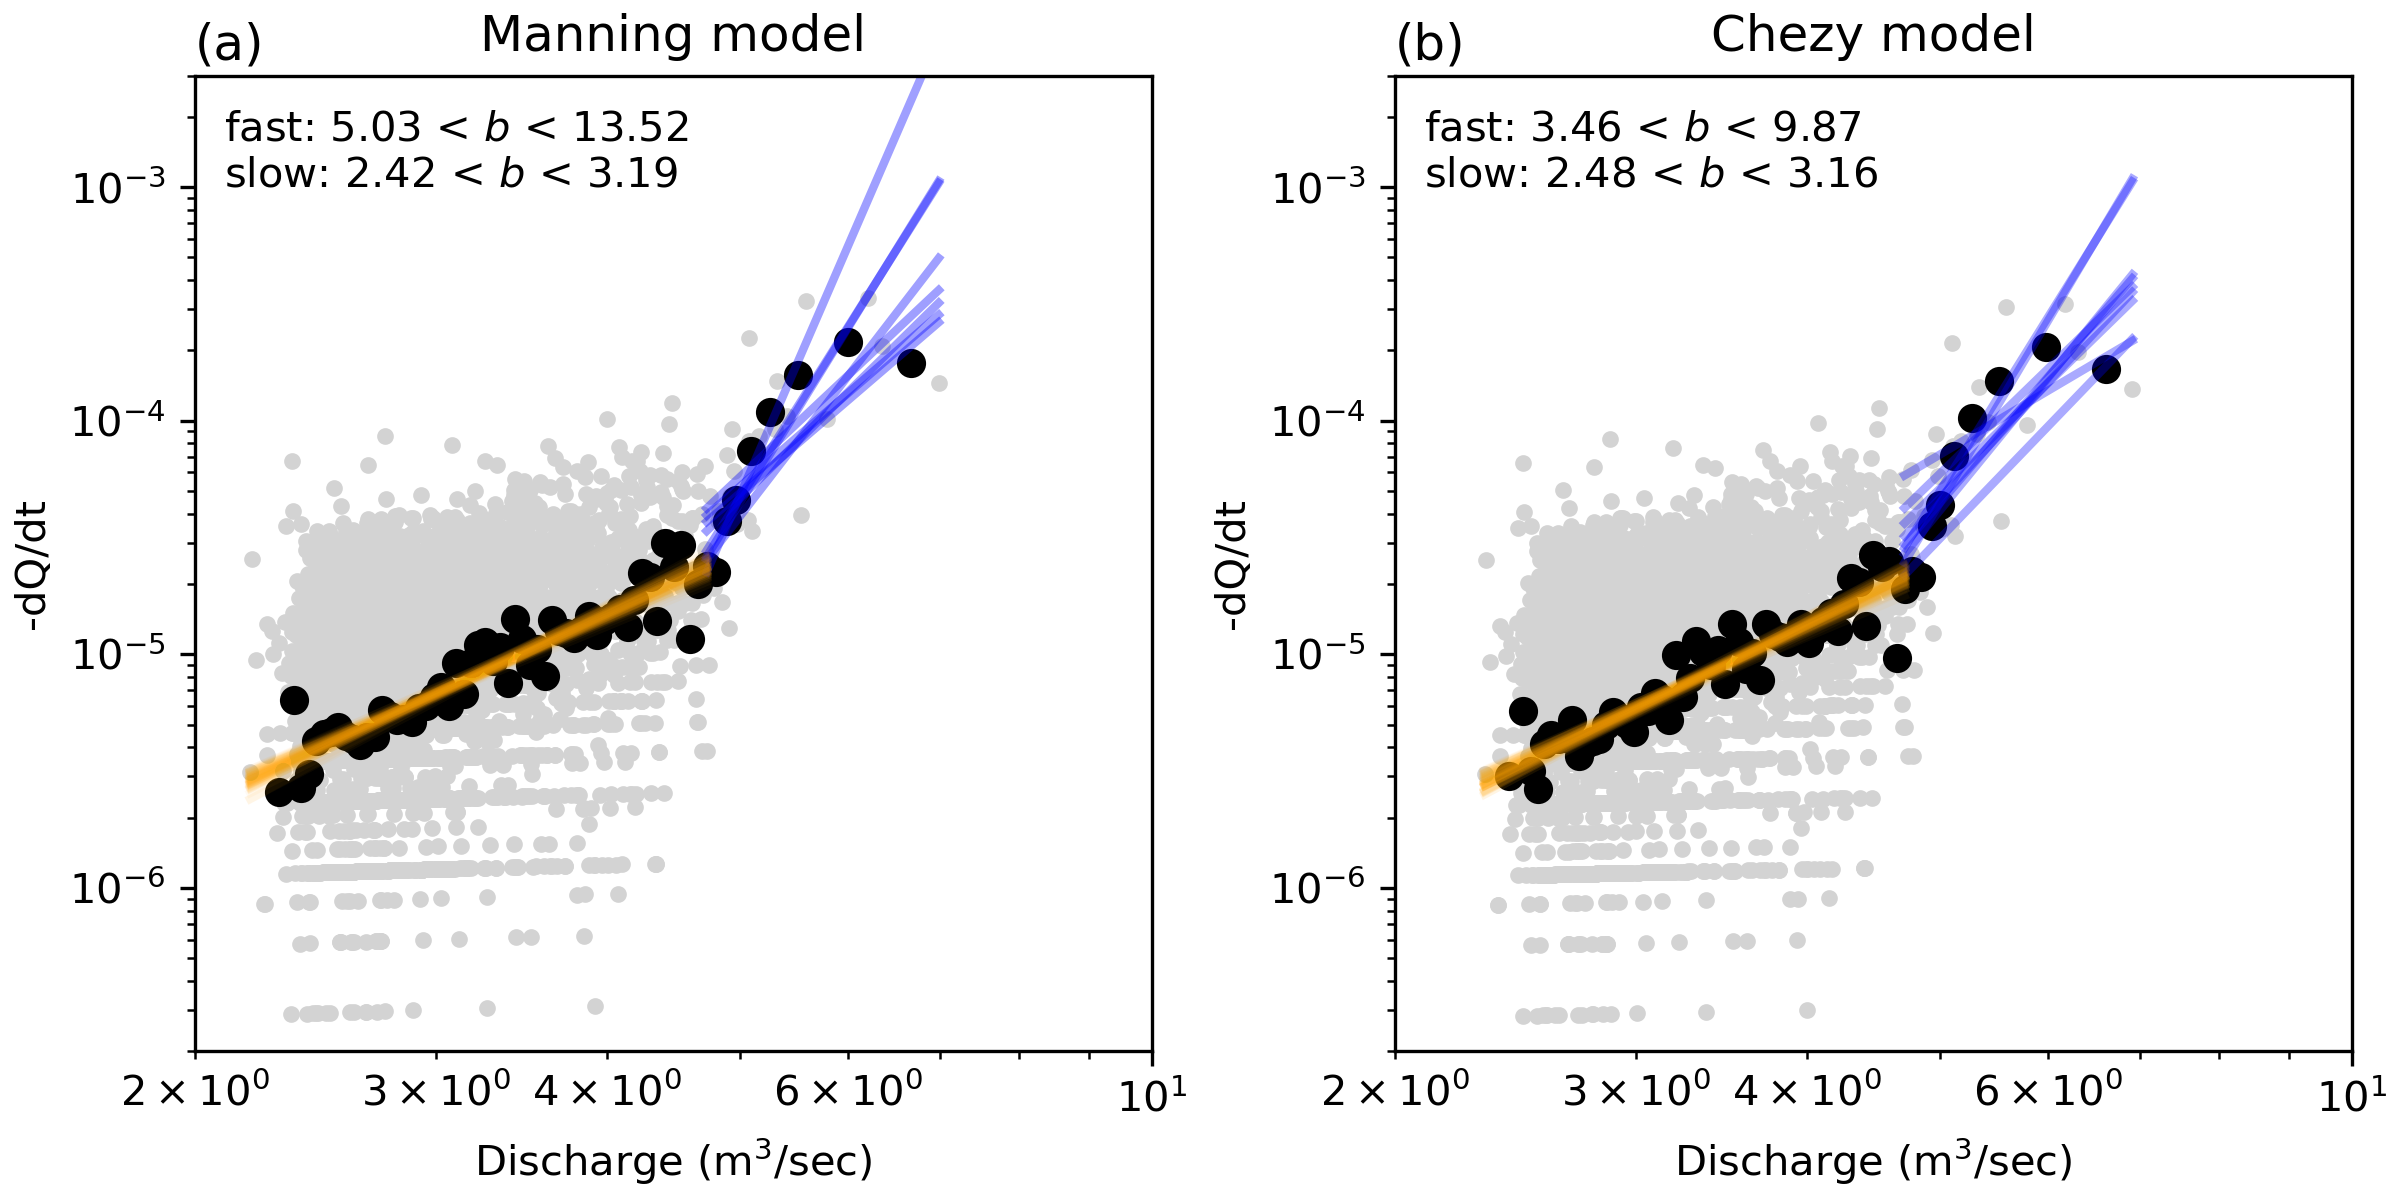
\includegraphics[width=.8\linewidth]{./figures/figure05.png}
\caption{Log-log plot of discharge against $-dQ/dt$ for the three post monsoon seasons from 2016 in the Kahule Khola catchment. The binned data is plotted in black, with the break in slope defining the transition from fast to slow-flow. A bootstrap method was used to estimate the range of the $b$ coefficient.}
\label{fg:recession}
\end{figure}

The late recession is consistently higher than model derived estimates for $b$ in steep compartmentalised systems \citep{rupp-2006,roques-etal-2022}. In comparison to the USGS data, the late recession value of $b$ is within the outliers (Figure \ref{fg:compare}). It is worth noting that within the USGS data high recession values are found for regions classified as semiarid mountains with impermeable soils and permeable bedrock \citep{tashie-etal-2020}. The early recession values are very high, significantly higher than those captured in the time-dependent modelling of discharge of a steep compartmentalised system \citep{roques-etal-2022} and likewise plot as an outlier against the USGS data (Figure \ref{fg:compare}).

\begin{figure}
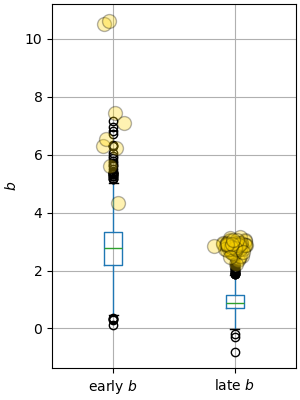
\includegraphics[width=5cm]{./figures/figure06.png}
\caption{Comparison of early and late recession values to USGS observations \citep{tashie-etal-2020}. The bar plot is for the USGS data, while the scattered yellow circles show the range of $b$ calculated form the bootstrap method (Figure \ref{fg:recession}).}
\label{fg:compare}
\end{figure}

\subsection{Modelling of compartmentalised flow}

Following the work of \cite{roques-etal-2022}, we explore if the high values of $b$ from early to late recession can be accounted for by compartmentalisation of the groundwater system within the Kahule Khola catchment. We focus on the model estimates of $b$, assuming that this is scale independent for a steep mountain catchment. The model domain is as described in Figure \ref{fg:domain}, and in the following section the impact of varying the thickness of the top high hydraulic conductivity layer, the topographic slope, and the change in hydraulic conductivity.

\subsubsection{Impact of compartmentalisation on recession trends}

The model is run with a precipitation rate of 0.5 mm/hr, which is equivalent to an total precipitation of 1500 mm over the four monsoon months. This precipitation lasts for 50 days such that the subsurface is saturated. Subsequently there is zero precipitation and water can seep out via the top model surface and the topmost section of the left hand boundary down to the depth of 10\,m (Figure \ref{fg:domain}. The recessing groundwater discharge is then plotted as $-dQ/dt$ against $Q$ in log-log space (e.g. Figure \ref{fg:varyD}a) and the gradient $b(Q)$ is calculated within the log-log space (e.g. Figure \ref{fg:varyD}b). The model resolves the nonlinear coupled equations for $h_{p}$ and $\theta$ using a Newton-Raphson scheme where if the solution fails to converge within a factor of $10^{-5}$, the time step is reduced until convergence is successful. Rather than explore the whole range of model parameters \citep[see][]{roques-etal-2022}, we focus on models that generate a late recession $b$ in the range $2.4 < b < 3.2$ (Figure \ref{fg:recession}).

\begin{figure}
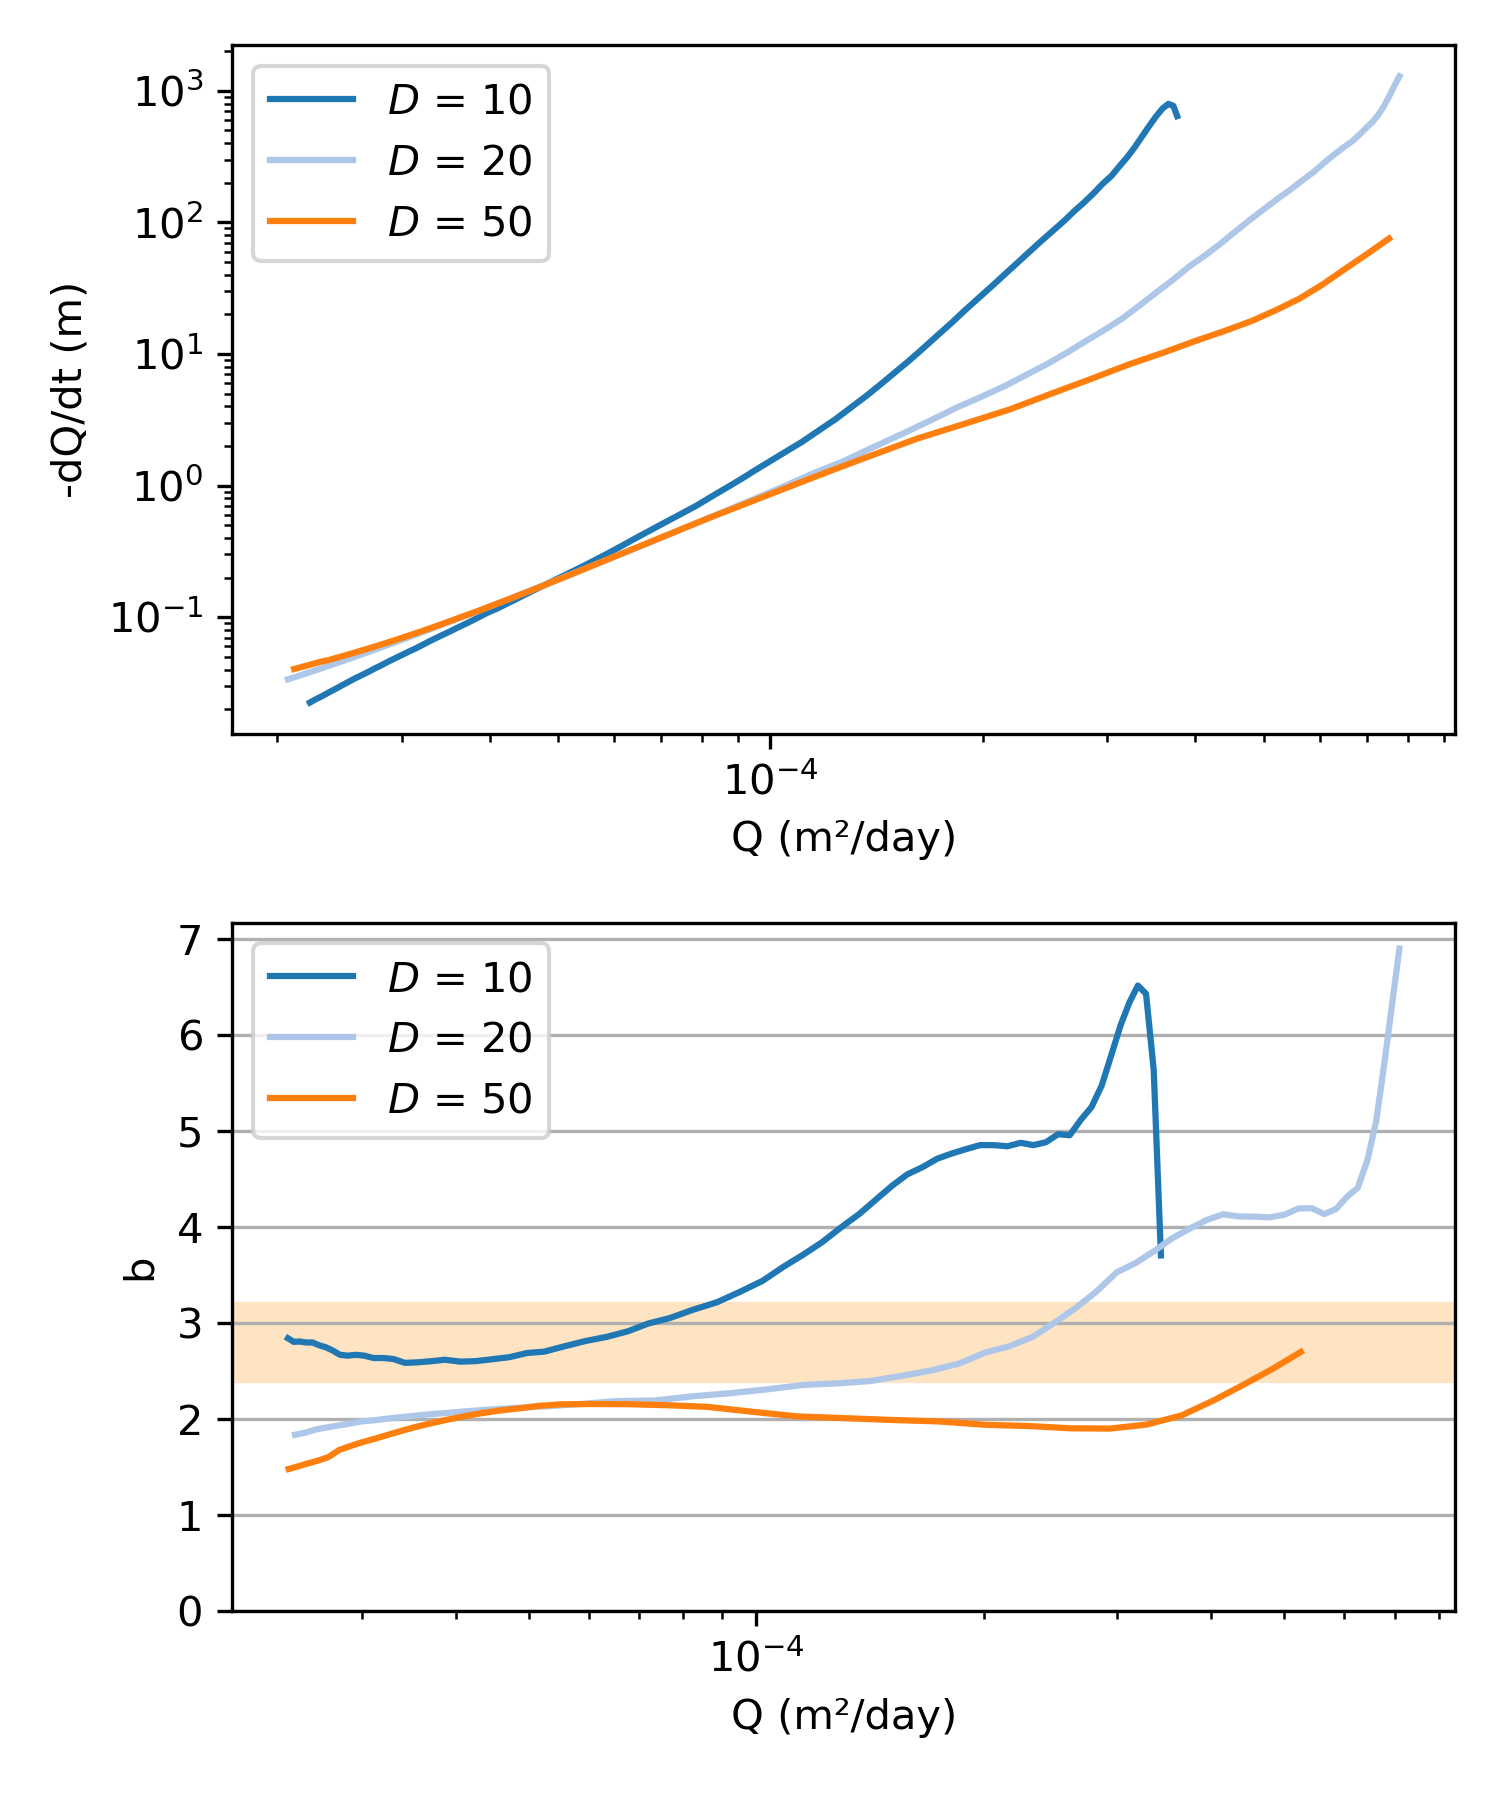
\includegraphics[width=.45\linewidth]{./figures/figure07.png}
\caption{Log-log plot of model recession for variations in $D$, with $\beta=0.3$ and $r_{K} = K_{U}/K_{0} = 64$. (a) Recession plot for three models of varying weathered layer thickness, $D = [10, 20, 50]\rm\,m$. (b) Variation in $b(Q)$ for the different values of $D$, where the gradient is calculated over a moving window of 10 model time steps to avoid errors due to time step magnitude reductions related to convergence. The bisque coloured bar represents the range of late recession $b$ from the discharge estimates (Figure \ref{fg:recession}).}
\label{fg:varyD}
\end{figure}

The recession trends for different thickness of the top weathered layer in general show an early recession with a higher slope than the late recession (Figure \ref{fg:varyD}). If the top weathered layer is thick, 50\,m thick, then the recession shows two phases, an early phase where $b$ ranges from 2.5 to 2, and then a late recession where $b$ trends towards 1.5. When the top weathered layer is 20\,m thick the recession show three phases. There is an initial brief very early recession with $b$ in excess of 4. Recession then transitions into an early recession with $b\sim4$. Subsequently the model tends towards a late recession with $b\sim2$. Finally if the top weathered layer is 10\,m thin then there is a similar three phase recession with an very early phase of $b>5$ and an early recession with $b\sim5$. The model then transitions to the late recession with $2.5 < b < 3.0$ (Figure \ref{fg:varyD}). Therefore if there is a thin weathered layer the late recession is within the range inferred from the Kahule Khola discharge estimates (Figure \ref{fg:recession}).

\begin{figure}
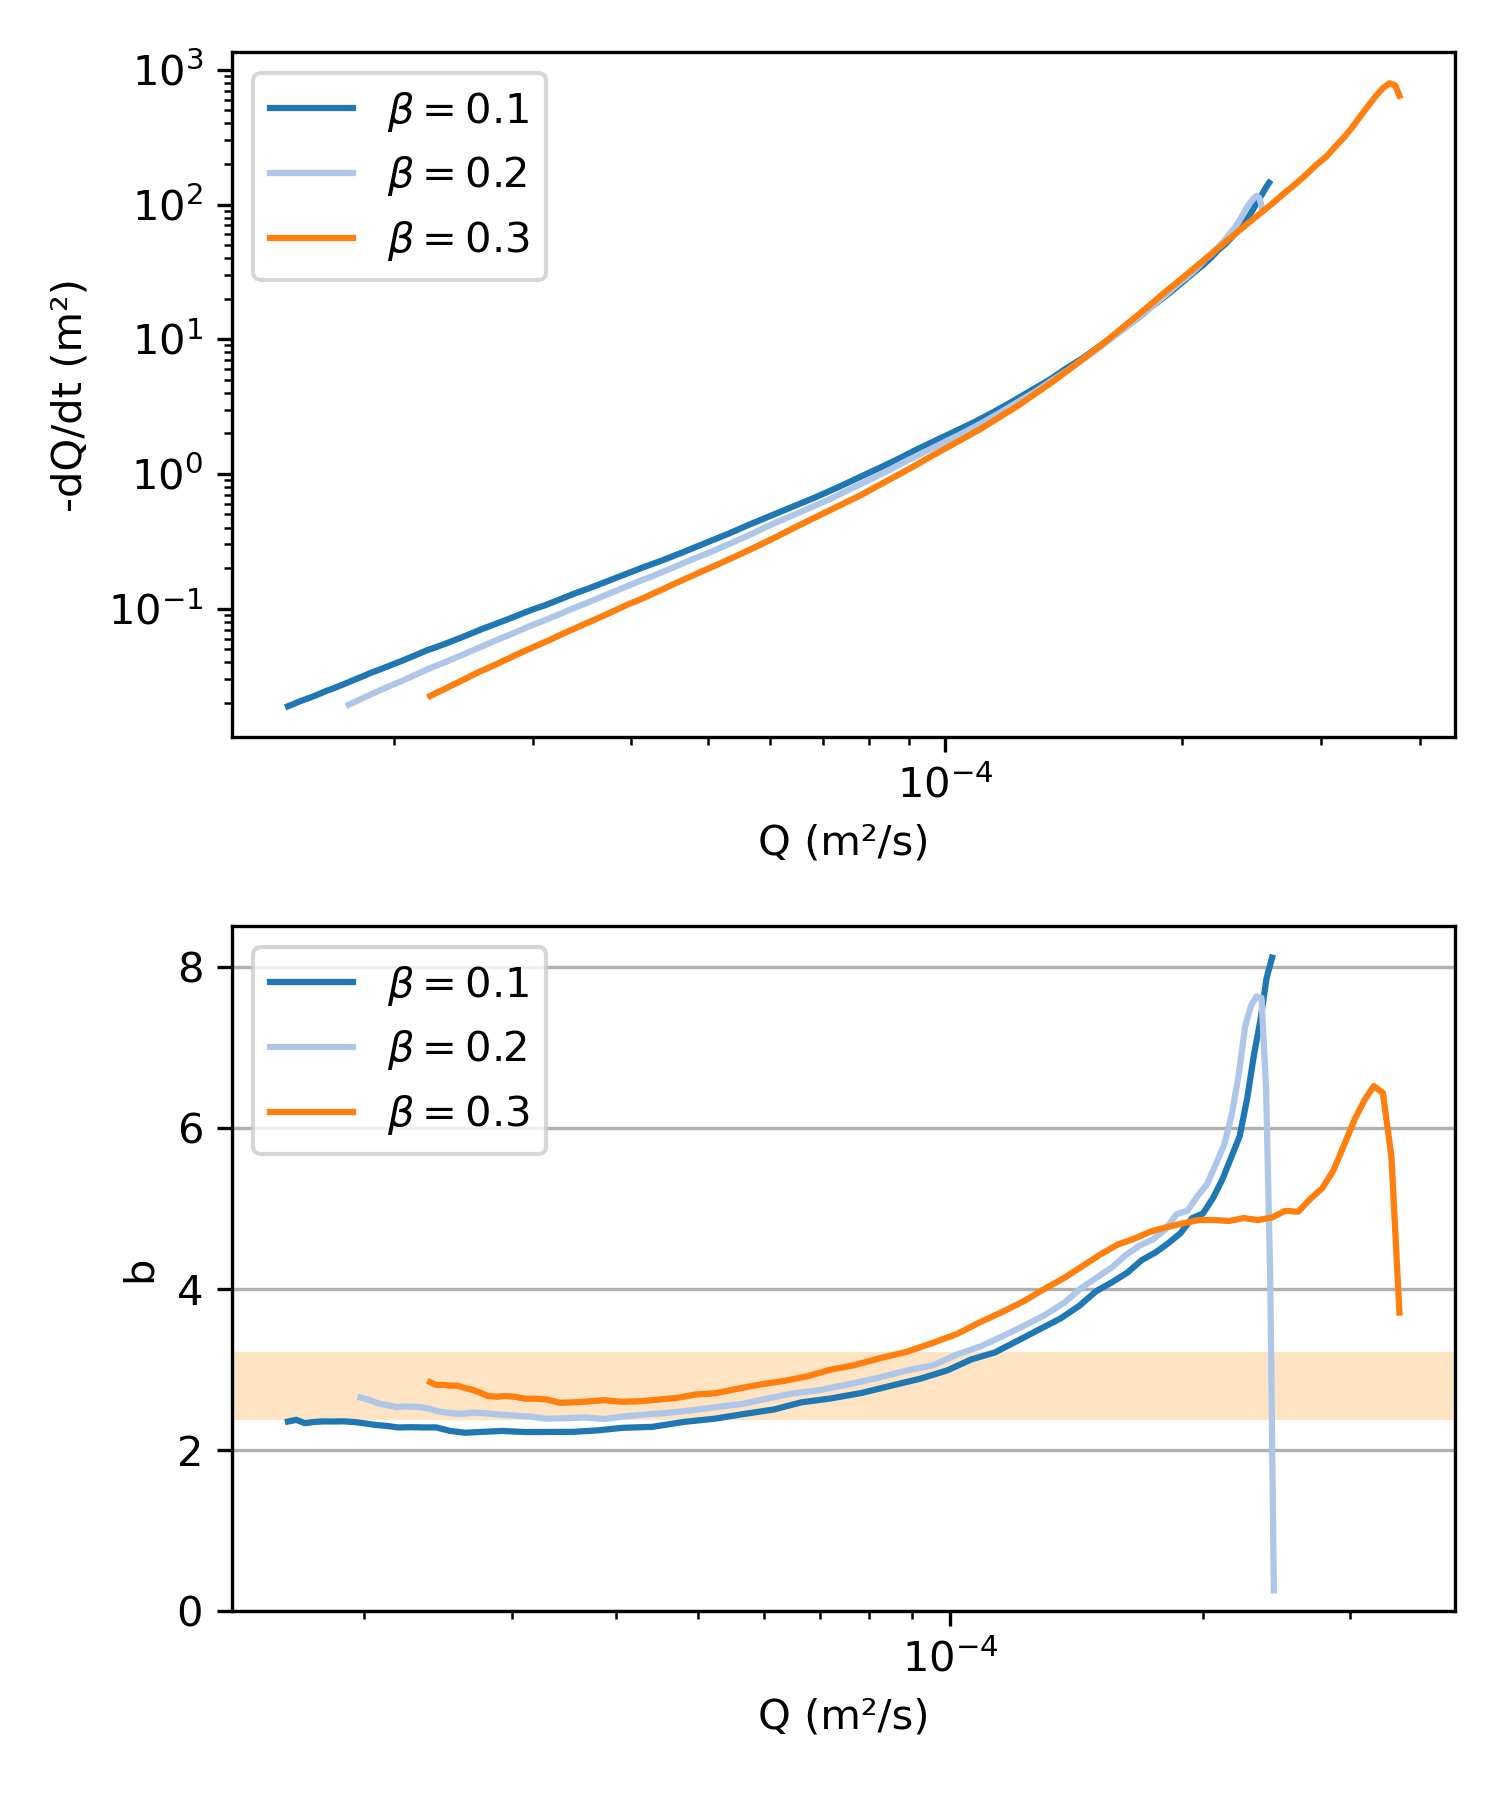
\includegraphics[width=.45\linewidth]{./figures/figure08.png}
\caption{Log-log plot of model recession for variations in $\beta$, with $D=10\rm\,m$ and $r_{K} = K_{U}/K_{0} = 64$. (a) Recession plot for three models of $\beta = [0.1, 0.2, 0.3]$. (b) Variation in $b(Q)$ for the different values of $\beta$, where the gradient is calculated over a moving window of 10 model time steps to avoid errors due to time step magnitude reductions related to convergence. The bisque coloured bar represents the range of late recession $b$ from the discharge estimates (Figure \ref{fg:recession}).}
\label{fg:varybeta}
\end{figure}

The three phase recession is only recovered for when the topographic slope is steep, $\beta>0.2$ (Figure \ref{fg:varybeta}). When $\beta\leq0.2$ and the model generates a $b(Q)$ relationship that is a gradual transition from high values reducing to $b\sim2$ (Figure \ref{fg:varybeta}). When the topographic slope is high there is however a sustained early recession. The magnitude of $b$ during the early recession is subsequently a function of the weathered layer thickness and the contrast in hydraulic conductivity between the top weathered layer and the lower fractured bedrock (Figure \ref{fg:varyrK}). For the same weathered layer thickness, 10\,m, and slope, $\beta=0.3$, an increase in the weathered layer hydraulic conductivity reduces the early recession $b$ (Figure \ref{fg:varyrK}). When $r_{K}$ is low the recession behaviour is more dominated by the top layer, where $b$ reduces to late recession values towards the end of the model discharge (Figure \ref{fg:varyrK}).

\begin{figure}
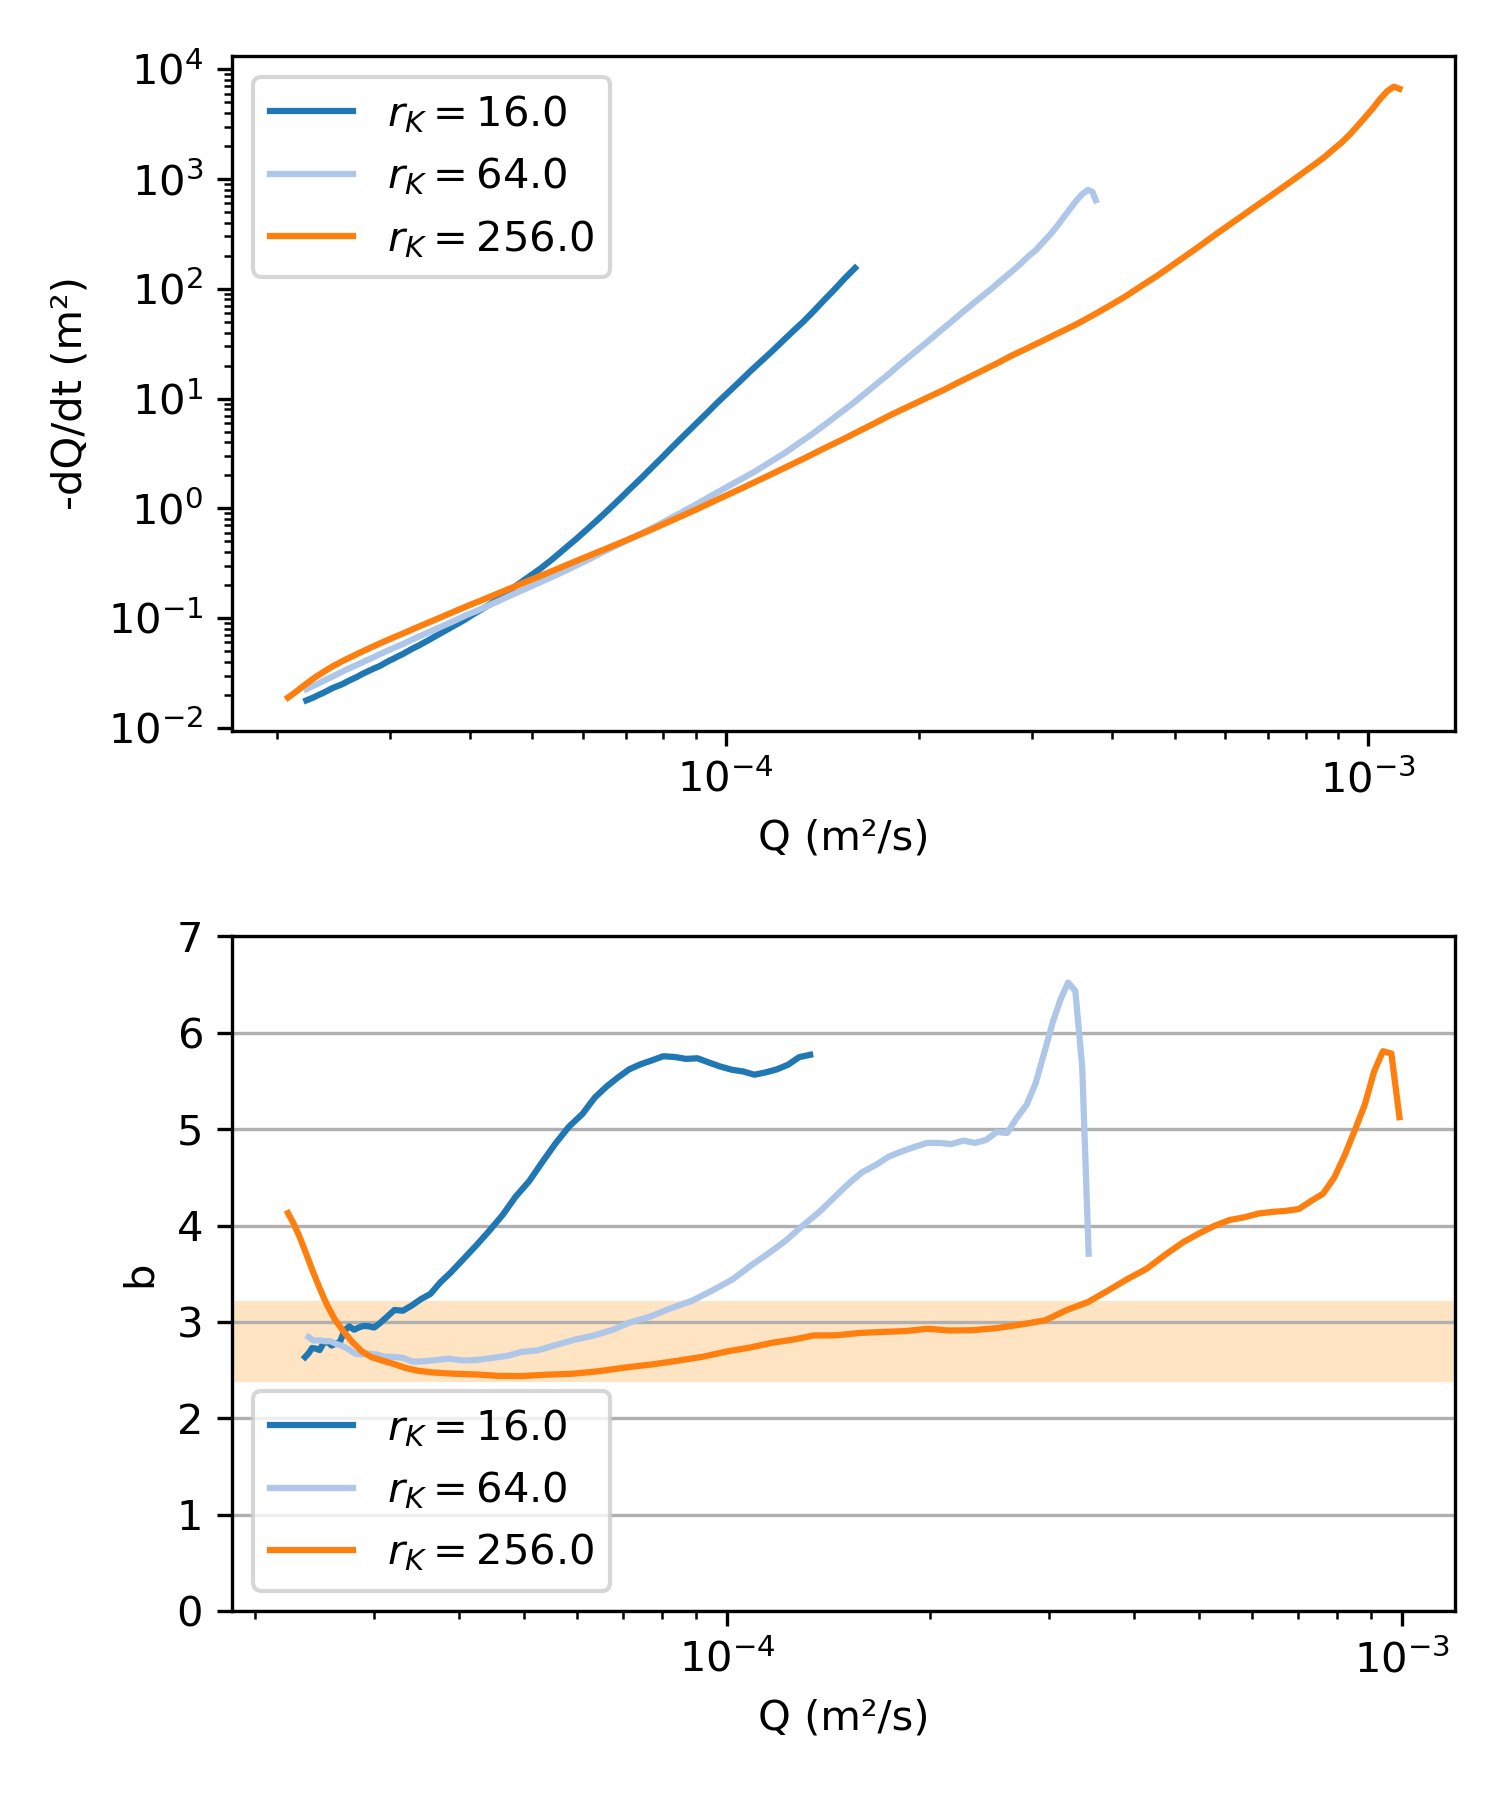
\includegraphics[width=.45\linewidth]{./figures/figure09.png}
\caption{Log-log plot of model recession for variations in $r_{K} = K_{U}/K_{0}$. (a) Recession plot for three models of varying weathered layer thickness, $K_{U} = [8\times 10^{-5}, 3.2\times 10^{-4}, 1.28\times 10^{-3}]\rm\,ms^{-1}$. (b) Variation in $b(Q)$ for the different values of $r_{K}$, where the gradient is calculated over a moving window of 10 model time steps to avoid errors due to time step magnitude reductions related to convergence. The bisque coloured bar represents the range of late recession $b$ from the discharge estimates (Figure \ref{fg:recession}).}
\label{fg:varyrK}
\end{figure}

\subsubsection{A best fit model to early and late recession}

\begin{figure}
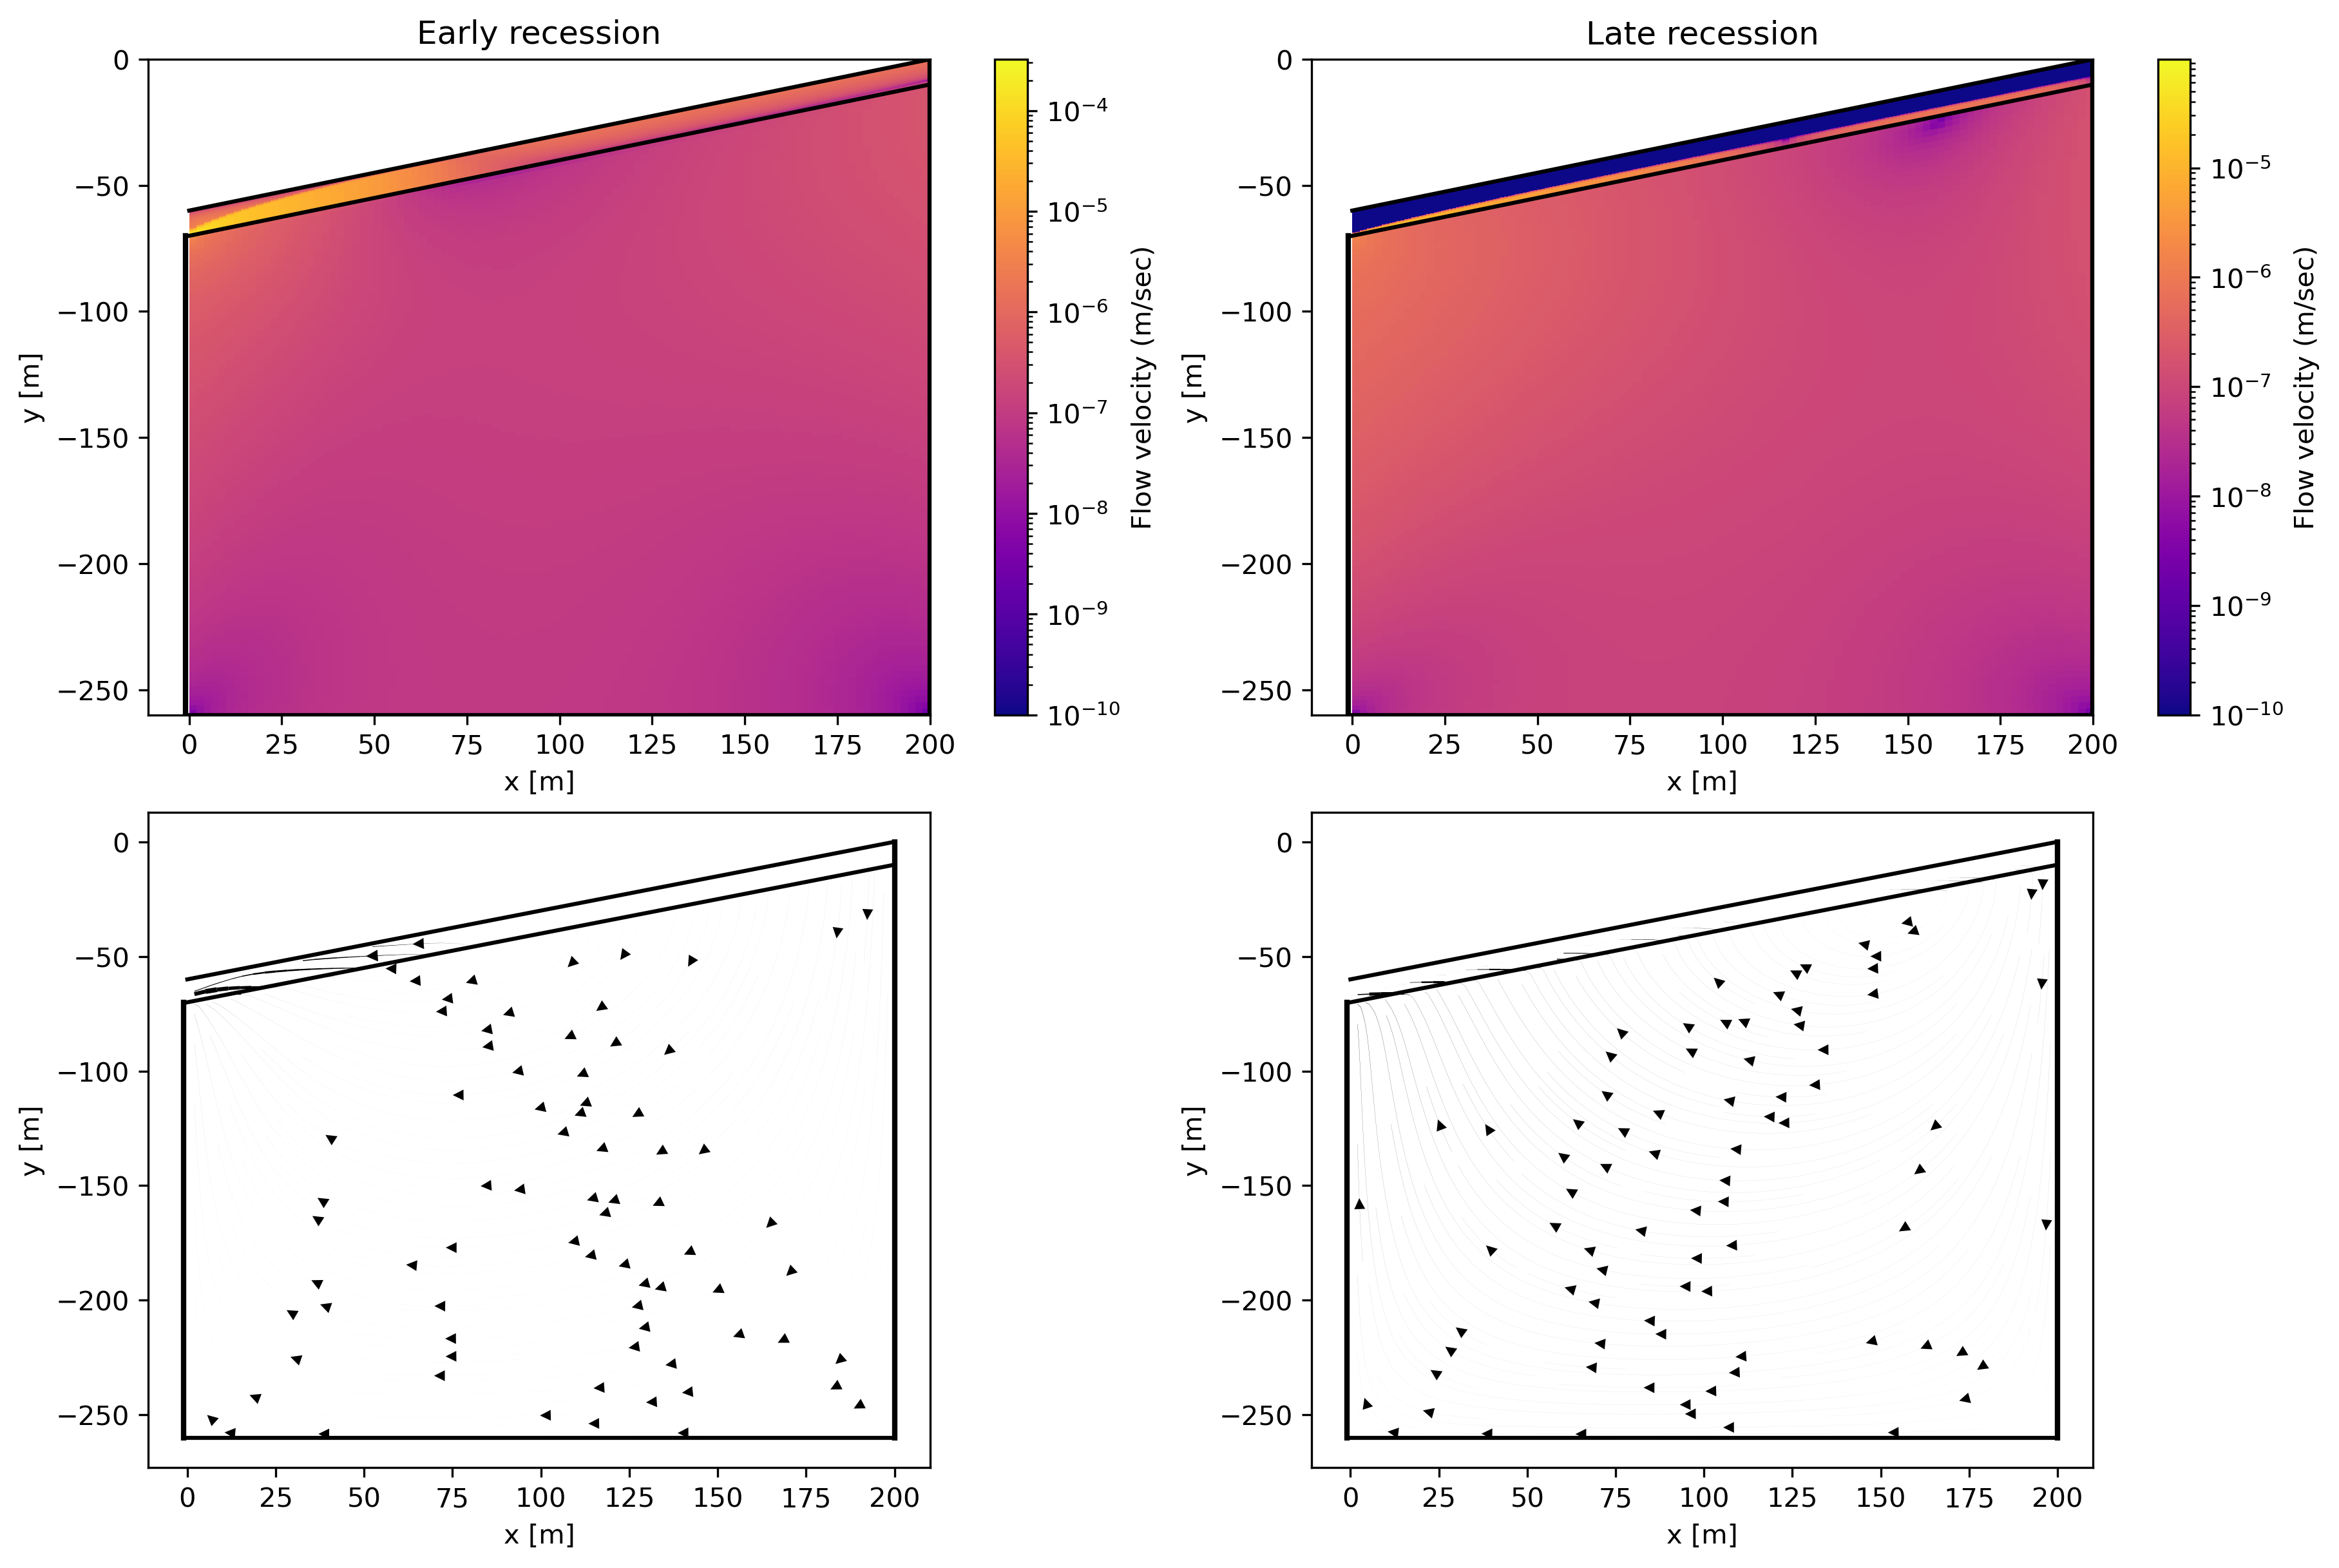
\includegraphics[width=0.8\linewidth]{./figures/figure10.png}
\caption{Groundwater flow during early and late recession. (a) Groundwater flow velocity magnitude during early recession, where the increased velocity within the top weathered layer can be seen. (b) Groundwater flow velocity magnitude during late recession, where the lower water table is visible. (c) Flow lines during early recession, where there is significant horizontal flow within the lower parts of the ot weathered layer. (d) Flow lines during late recession, showing a greater input from the deeper return flow.}
\label{fg:fast-slow-model}
\end{figure}

From the recession analysis and the model scenarios, a model with $D=10\rm\,m$, $\beta=0.3$ and $r_{K} = K_{U}/K_{0} = 64$ gives a $b(Q)$ that matches the estimates of the early and late recession from the discharge estimates. Flow lines and velocity magnitudes are plotted for instances during early and late recession (Figure \ref{fg:fast-slow-model}). During early recession the velocity magnitude is high within the top weathered layer and increases to around $10^{-4}\rm\,m\,s^{-1}$ at the outlet. Velocity magnitudes within lower fractured bedrock layer are of the order $10^{-6}\rm\,m\,s^{-1}$. The flow is in general horizontal within the weathered layer, with flow lines tracking the top of the water table towards the outlet (Figure \ref{fg:fast-slow-model}a and c). During late recession the water table descends to the base of the weathered layer and the groundwater flow is dominated by deep flow lines that flow through the fractured bedrock layer (Figure \ref{fg:fast-slow-model}a and c).

\subsection{Implications for groundwater dynamics in steep mountain catchments}

The results presented within this study align with previous work showing the importance of vertical permeability contrasts and compartmentalisation \citep{roques-etal-2022}. $r_{K} > 1$ generates flow compartmentalisation while increasing $D$ will dampens the effects of compartmentalisation on the recession. They reinforce the idea that realistic representations of flow regimes in mountainous environments require explicit modelling of dual domains. In the context of resource management, our findings suggest that neglecting structural contrasts may lead to misrepresentation of recession and storage dynamics, particularly for applications involving baseflow prediction, low flow forecasting, or groundwater recharge assessments. This is especially critical in fractured catchments like Kahule Khola where weathering depth and topographic gradients control seasonal flow partitioning.

These results support the idea that slow flow compartments are activated only when slope, contrast, and depth jointly allow sufficient storage and delayed drainage. In Kahule Khola, the simulated recession responses are not transient but appear structurally controlled, consistent with observations in deeply weathered hillslopes and saprolite mantled terrains \citep{rempe-2018,dralle-etal-2023}. More broadly, the simulations demonstrate that recession segmentation in can serve as a diagnostic indicator of subsurface compartmentalisation and flow regime organisation, even in the absence of explicitly modelled fractures or lateral heterogeneity. While this study is limited to vertically layered structures in 2D, the emergence of dual flow regimes suggests that structural contrasts alone can govern baseflow dynamics. Future work should incorporate discrete fracture networks and 3D heterogeneity to refine these interpretations and assess their robustness across geological contexts \citep{klos-etal-2018,carroll-etal-2025}.

\section{Conclusions}


\bibliographystyle{copernicus}
\bibliography{./main.bib}
\end{document}
